As we change the problem from a finite and known number of process with at most one biggest common ancestor (BCA) to an unknown number of processes with no restriction on the number of BCA, it is important to study what will change and what do we have to expect regarding the number of BCA. Therefore using a DAG random generator (see section~\ref{sec:daggen}) we started by implementing the same algorithm that the one used on a finite and known number of process, except that we now assume that each node $a$ of the DAG contains a hash $h(a)$ of size $k$. We label every node $a$ of the tree with a vector $v(a)$ such that $v(a)_i=\sum_{b\in \mathrm{ancestor}(a)} h(b)_i$, with this labeling we test wether the proposition \ref{propmin} can still be used in some way. From the definition of the labeling we have :
\begin{proposition}
 If $c$ is a biggest common ancestor of $a$ and $b$ then $v(c) \leq \mathrm{min}(v(a),v(b))$. \label{propinf}
\end{proposition}
In our Dag algorithm nodes are placed in different layers, each layers having links only with the previous and the next one. An important parameter to consider is the probability for a node that a node from the previous layer is one of its parents. Examples of the influence of this parameter (called $p$) can be found in section~\ref{sec:daggen}. The "high" of a DAG is the length of the biggest path between two nodes of the DAG. The next graphs show the influence of $p$ and the high of the DAG on the number of BCA and on the number of element verifying the proposition \ref{propinf}.
\begin{figure}[H]
  \centering
 \begin{subfigure}[b]{0.49 \textwidth}
  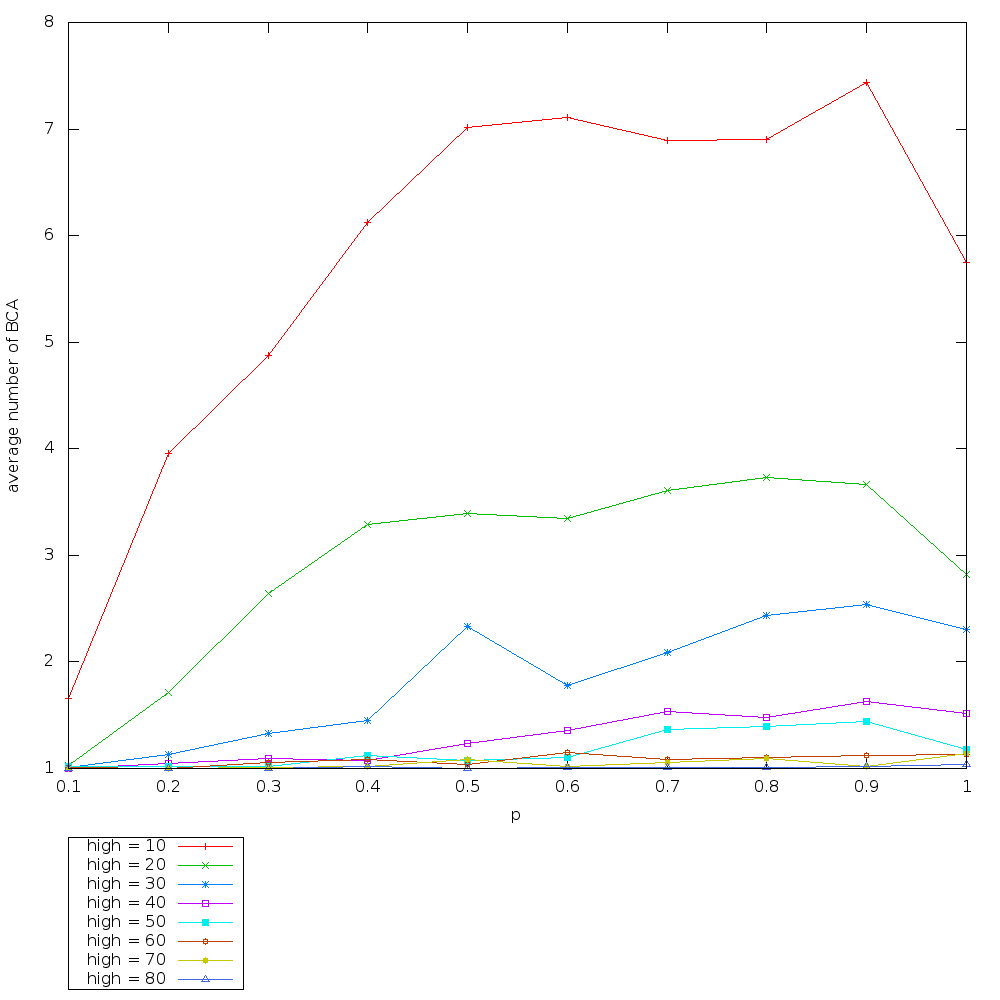
\includegraphics[width = \textwidth]{./image/resultprelim/averagenbbca.png}
  \caption{Number of Biggest Common Ancestor in a DAG with 100 nodes} \label{fig:nbbca}
 \end{subfigure}
 \begin{subfigure}[b]{0.49 \textwidth}
  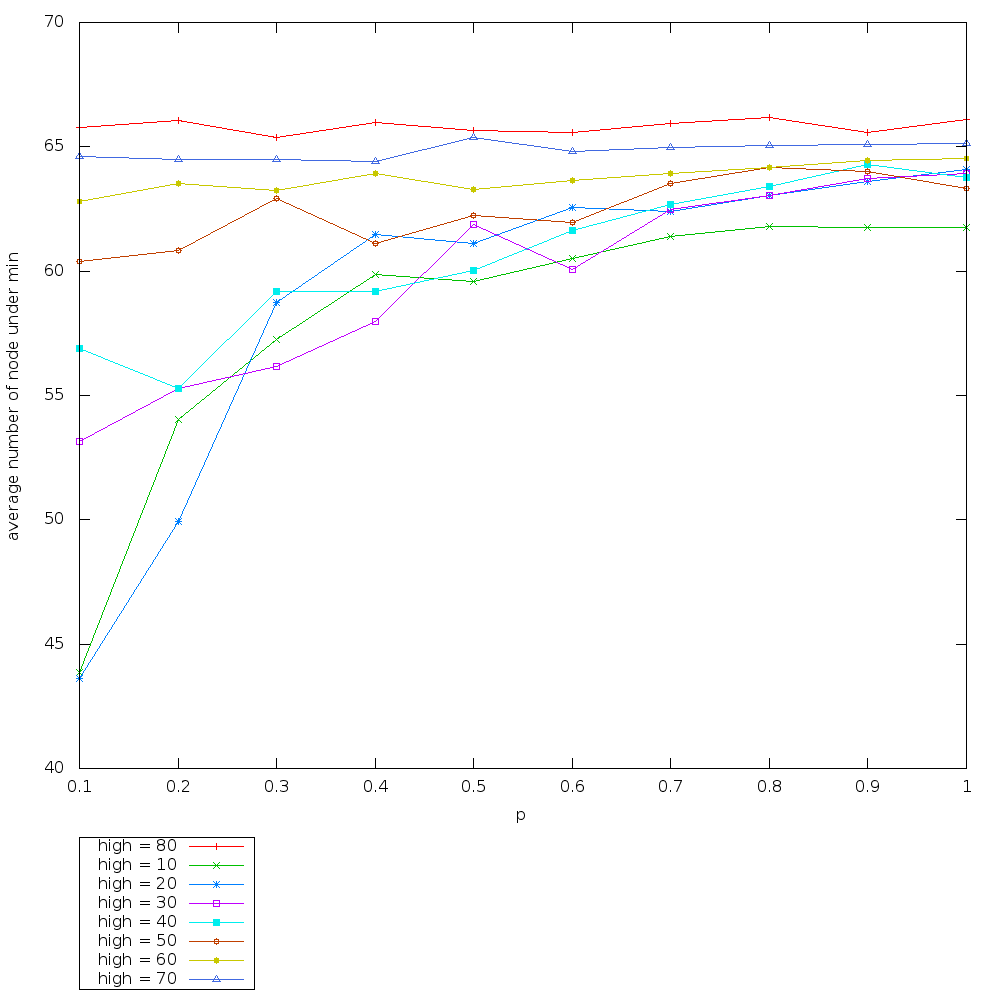
\includegraphics[width = \textwidth]{./image/resultprelim/averagenum.png}
  \caption{Number of element verifying the inequality of \ref{propinf} in a DAG with 100 nodes} \label{fig:num}
 \end{subfigure}
\end{figure}

Figure~\ref{fig:nbbca} underlines that the assumption on the number of biggest common ancestors was a strong assumption and that we can not rely on the case where there is only one BCA. Figure~\ref{fig:num} shows that adapting the algorithm from the case where we only have a finite and known number of processes might not be a good idea. Indeed we reduce the search of the biggest comman ancestor to $\frac{1}{3}$ of the DAG, but the size of the area to search remains linear in the size of the complete DAG.
